
%(BEGIN_QUESTION)
% Copyright 2011, Tony R. Kuphaldt, released under the Creative Commons Attribution License (v 1.0)
% This means you may do almost anything with this work of mine, so long as you give me proper credit

This Allen-Bradley MicroLogix 1000 PLC controls the energization of an electric motor and a lamp:

$$\includegraphics[width=15.5cm]{i02536x01.eps}$$

Sketch the necessary wire connections showing how to use the multimeter as a ``jumper'' to simulate the upper pushbutton switch being pressed, even if the actual switch is unpressed.  Assume you do {\it not} have access to the screw terminals on the switch itself, but only to terminals on the PLC.  Be sure to sketch the test leads extending all the way between the proper points in the PLC/switch circuit and the proper jacks on the meter itself!

\underbar{file i02536}
%(END_QUESTION)





%(BEGIN_ANSWER)

{\it Half-credit for proper meter test lead connections (to the PLC or to the corresponding terminal block terminals), and half-credit for proper meter jack connections (between ``A'' and ``COM'' on the meter):}

$$\includegraphics[width=15.5cm]{i02536x02.eps}$$

%(END_ANSWER)





%(BEGIN_NOTES)

{\bf This question is intended for exams only and not worksheets!}.

%(END_NOTES)

